\section{Central dogma of molecular biology}

\begin{figure}[H]
    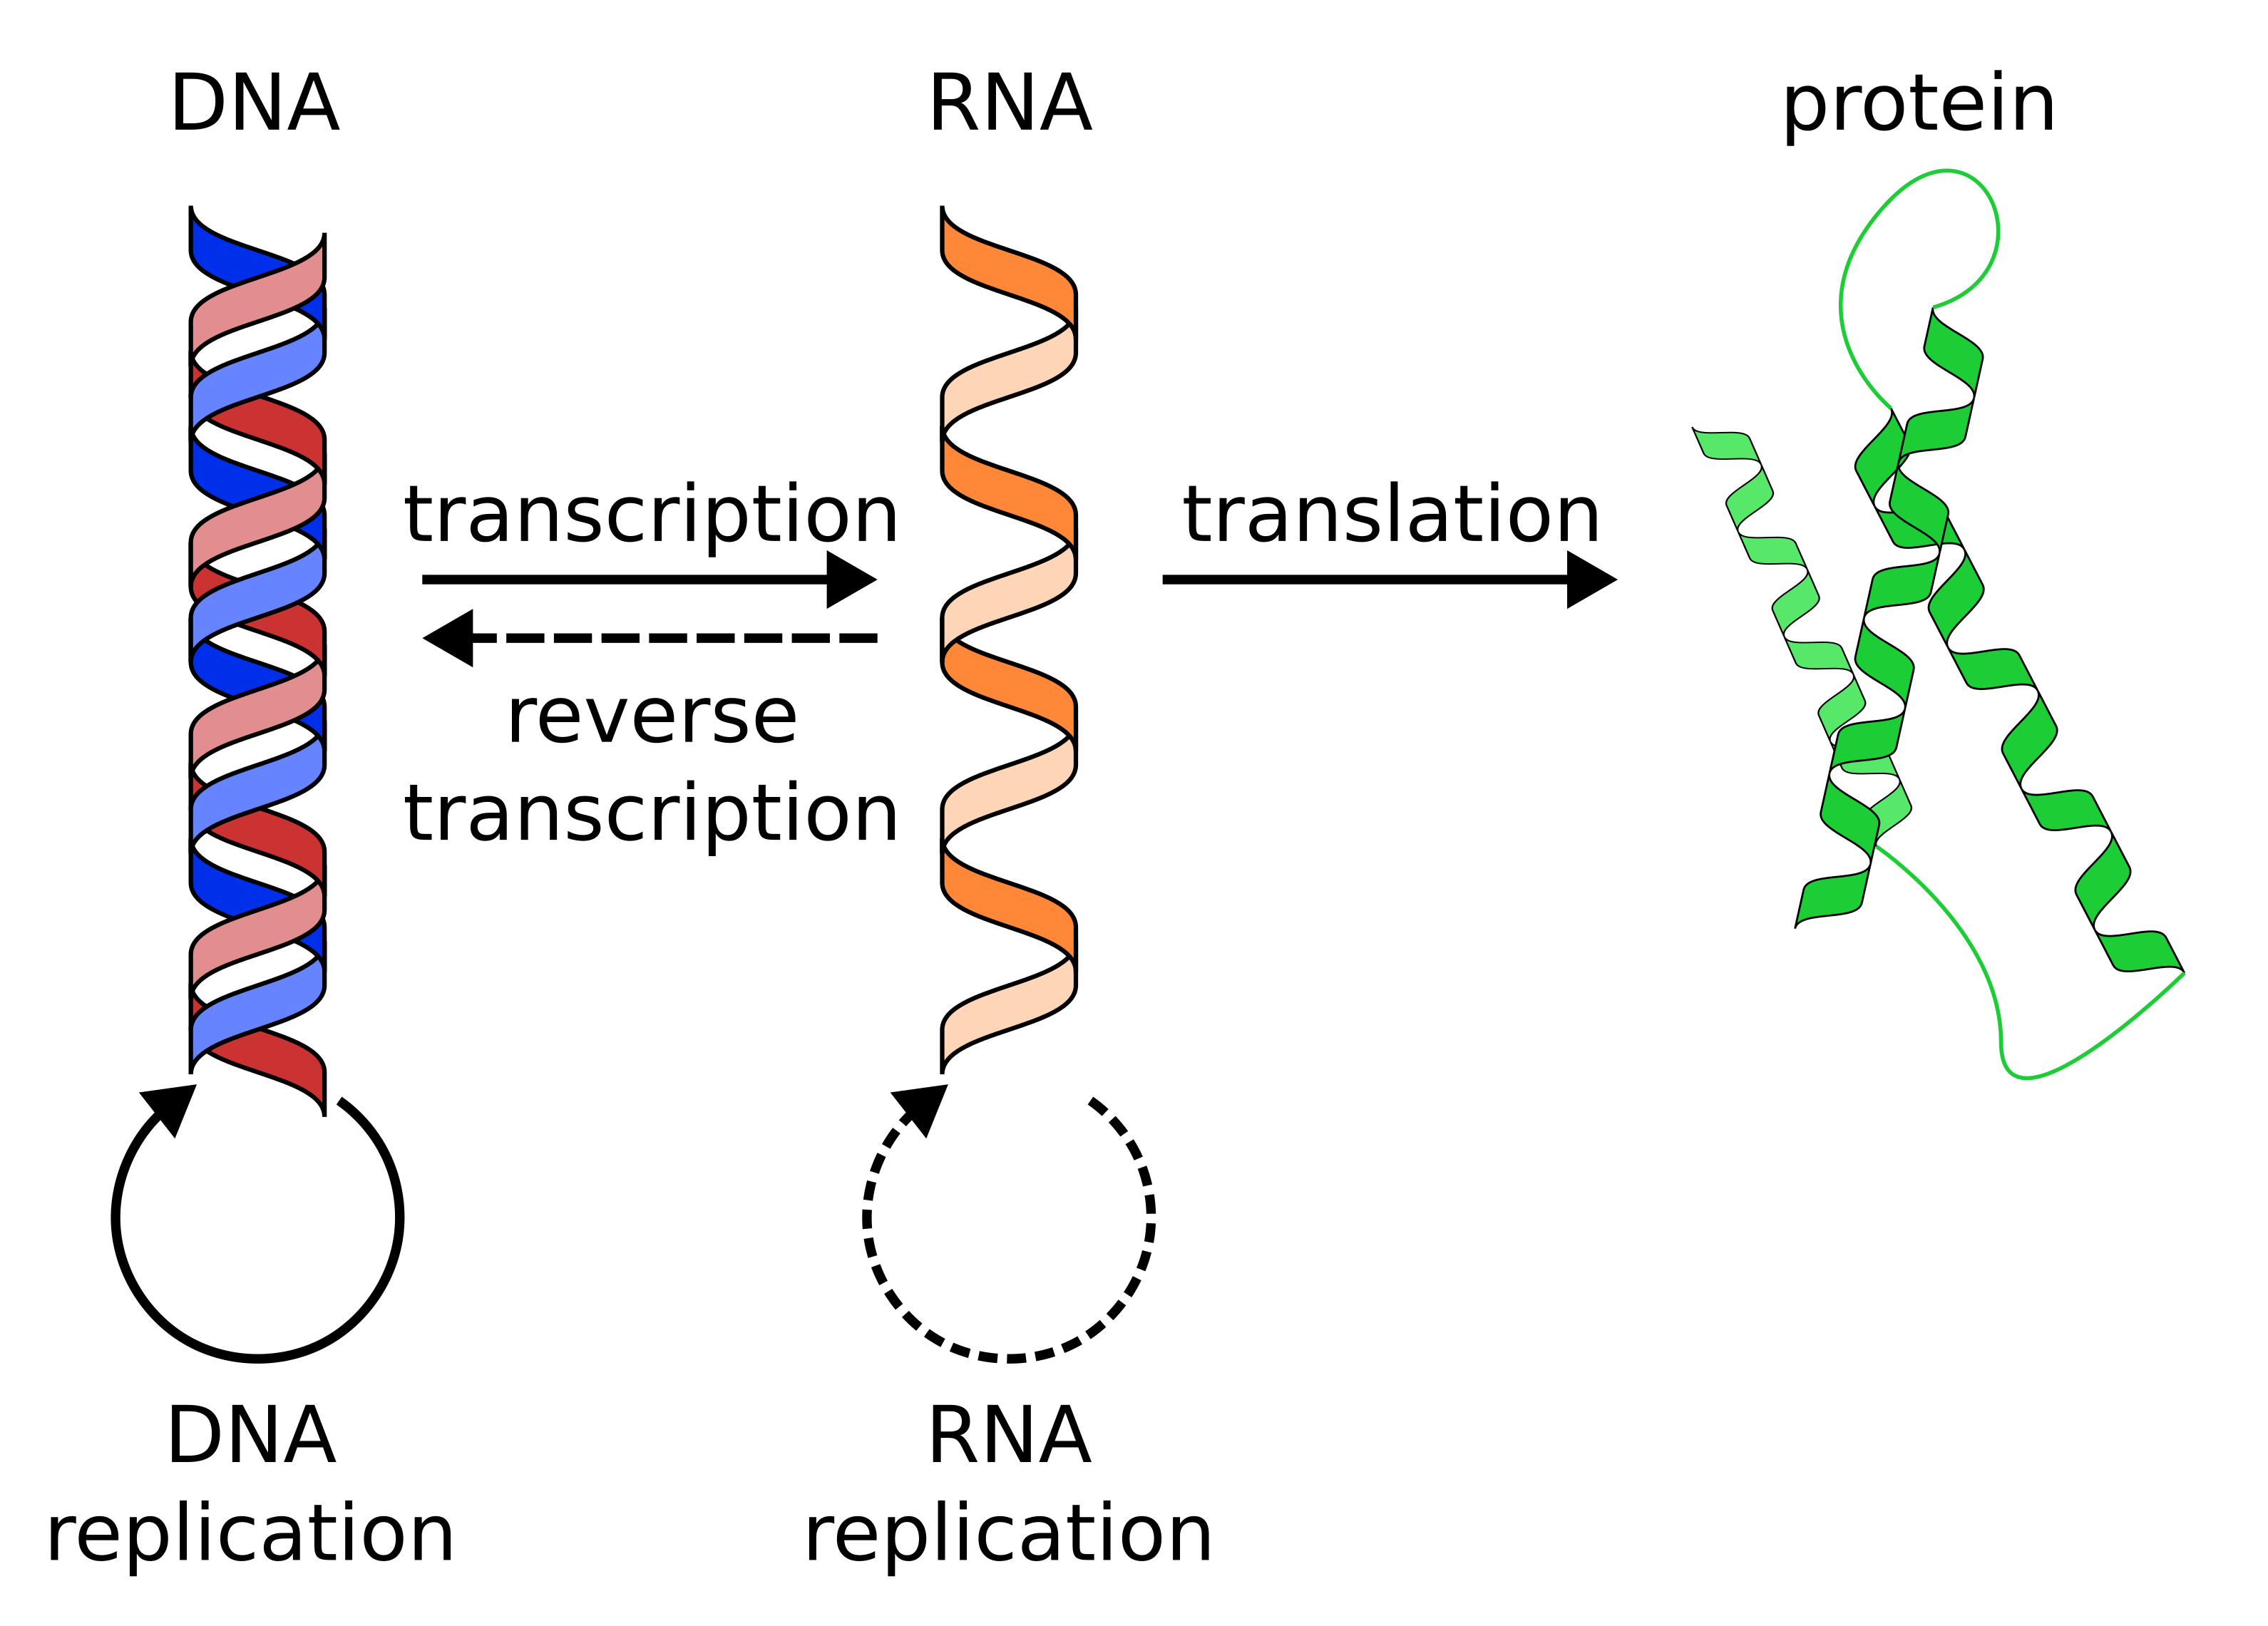
\includegraphics[width=\linewidth]{ch1.Introduction/imgs/central_dogma.png}
    \caption{Caption}
    \label{fig:central_dogma}
\end{figure}

\subsection{Transcription}

\begin{figure}[hbtp]
    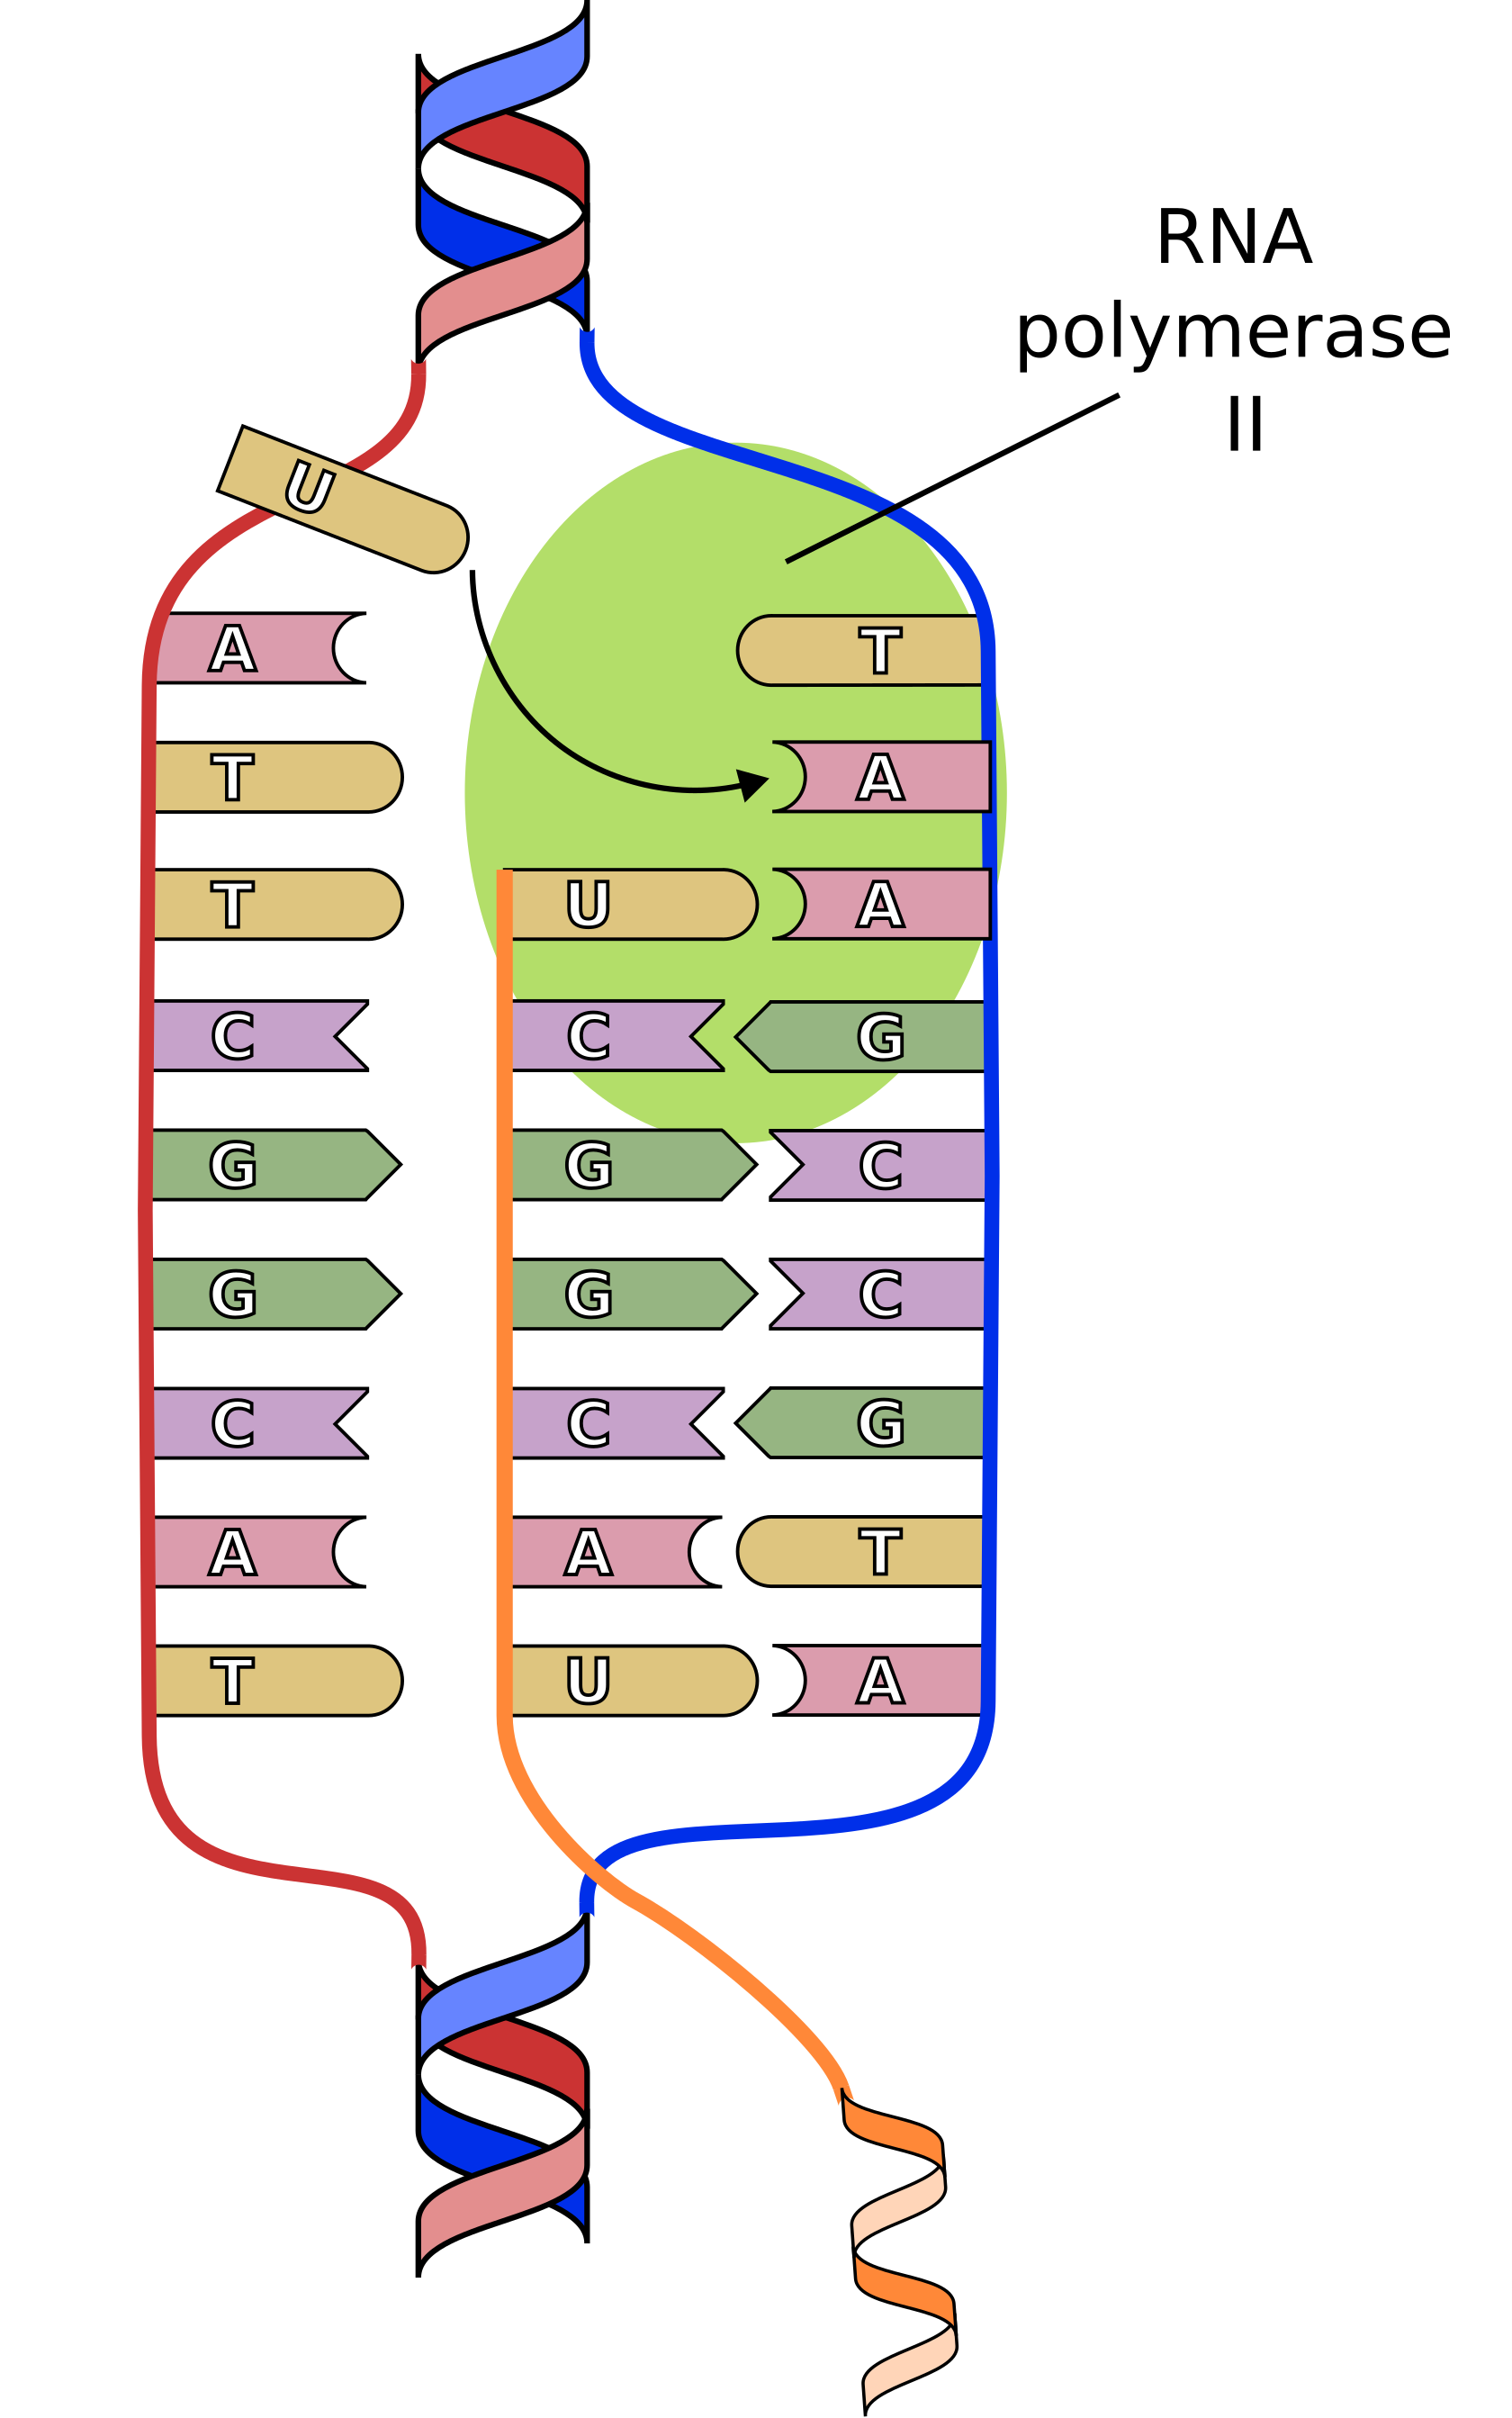
\includegraphics[height=0.9\textheight]{ch1.Introduction/imgs/transcription.png}
    \caption{Caption}
    \label{fig:transcription}
\end{figure}

\subsection{Translation}

\begin{figure}[H]
    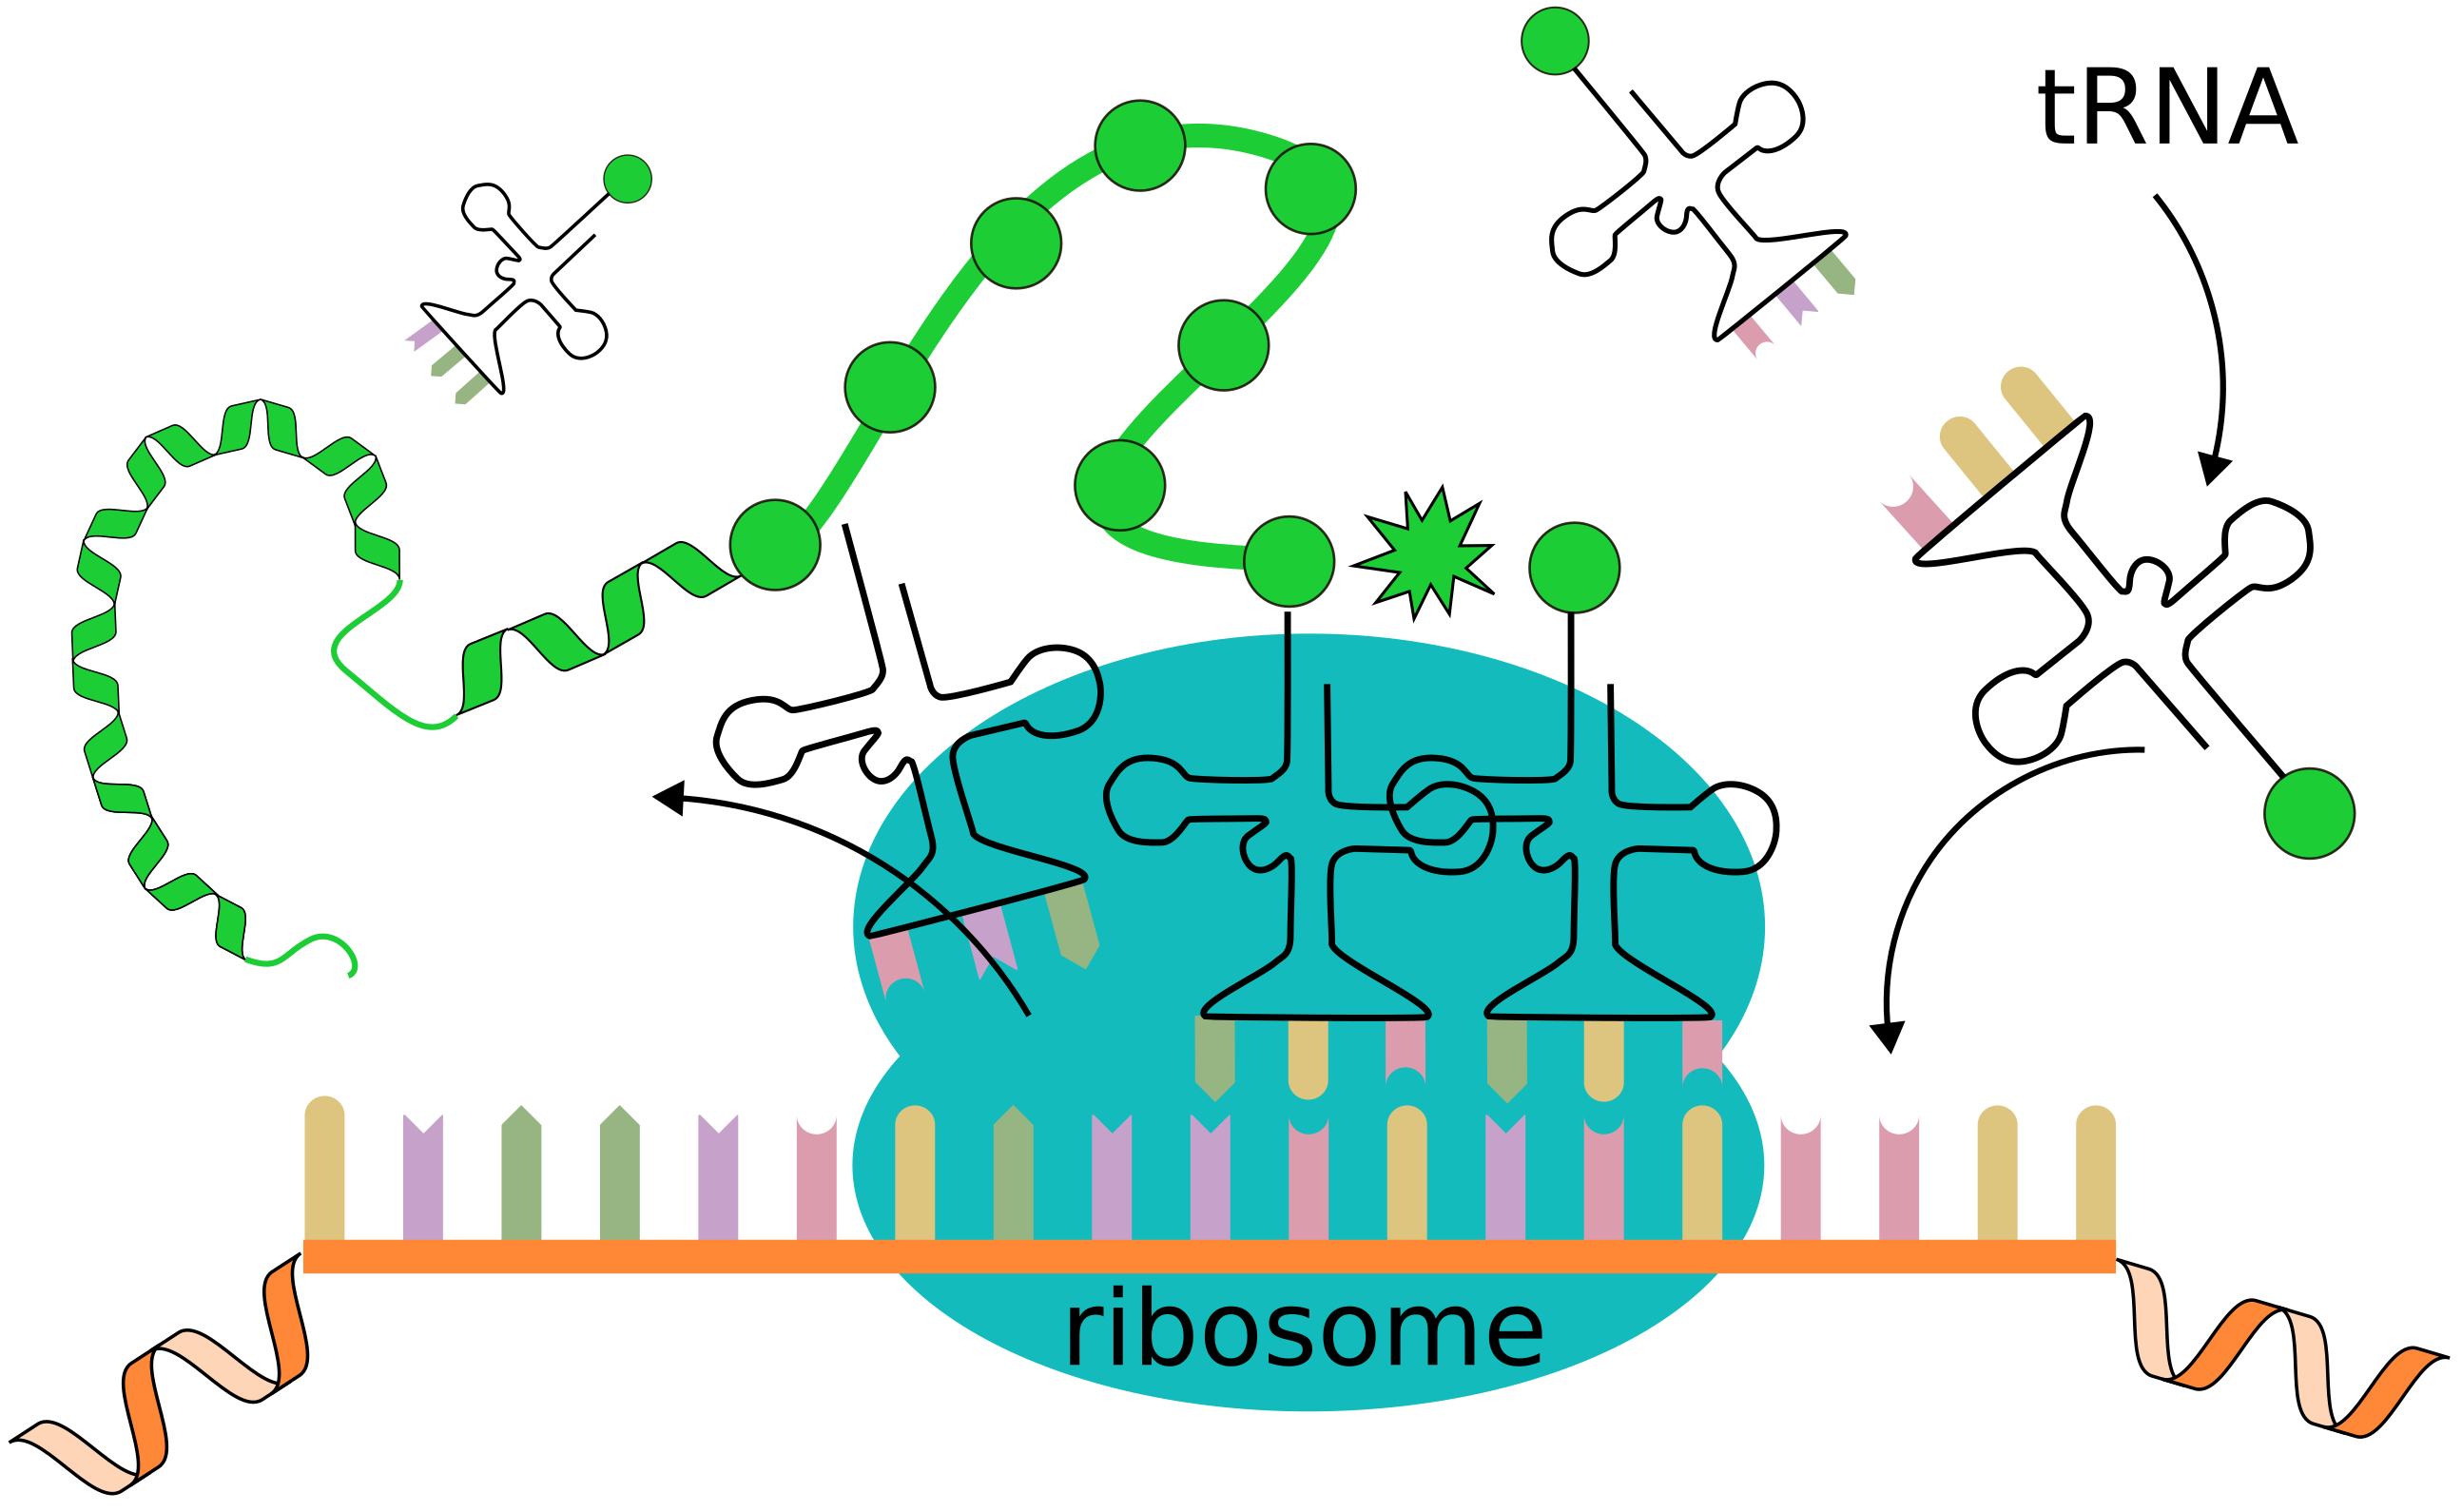
\includegraphics[width=\linewidth]{ch1.Introduction/imgs/translation.png}
    \caption{Caption}
    \label{fig:translation}
\end{figure}

\subsection{Chromatin}

\begin{figure}[H]
    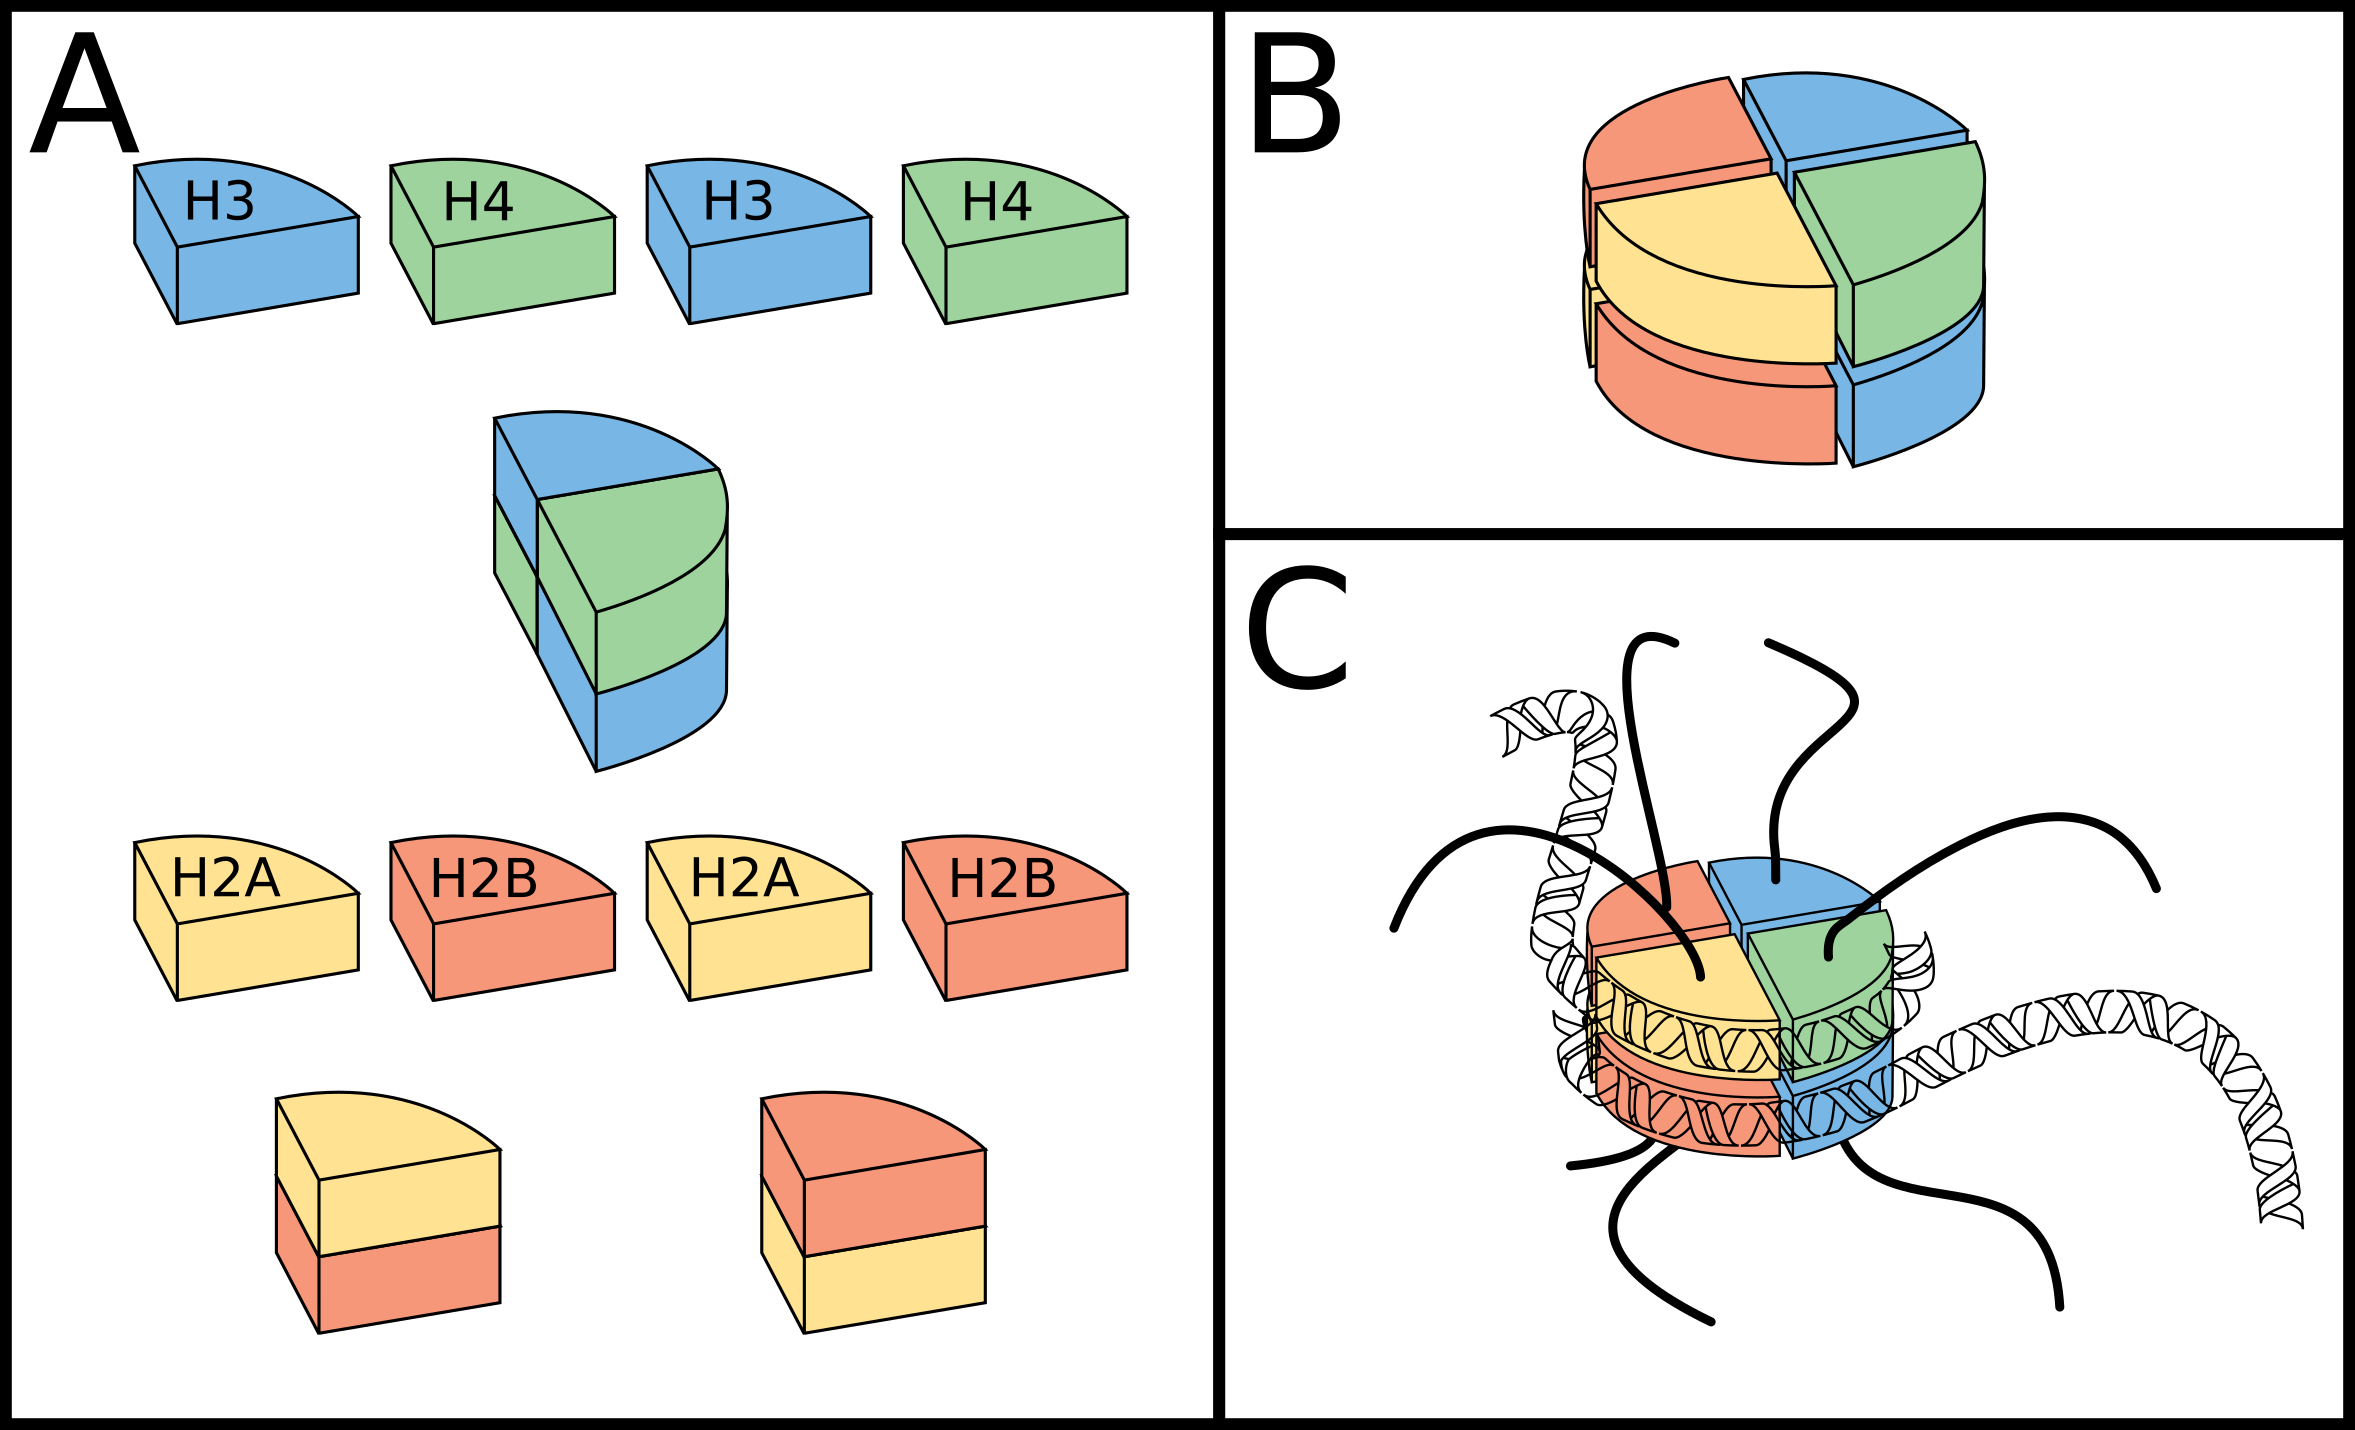
\includegraphics[width=\linewidth]{ch1.Introduction/imgs/histones.png}
    \caption{Caption}
    \label{fig:histones}
\end{figure}

\begin{figure}[hbtp]
    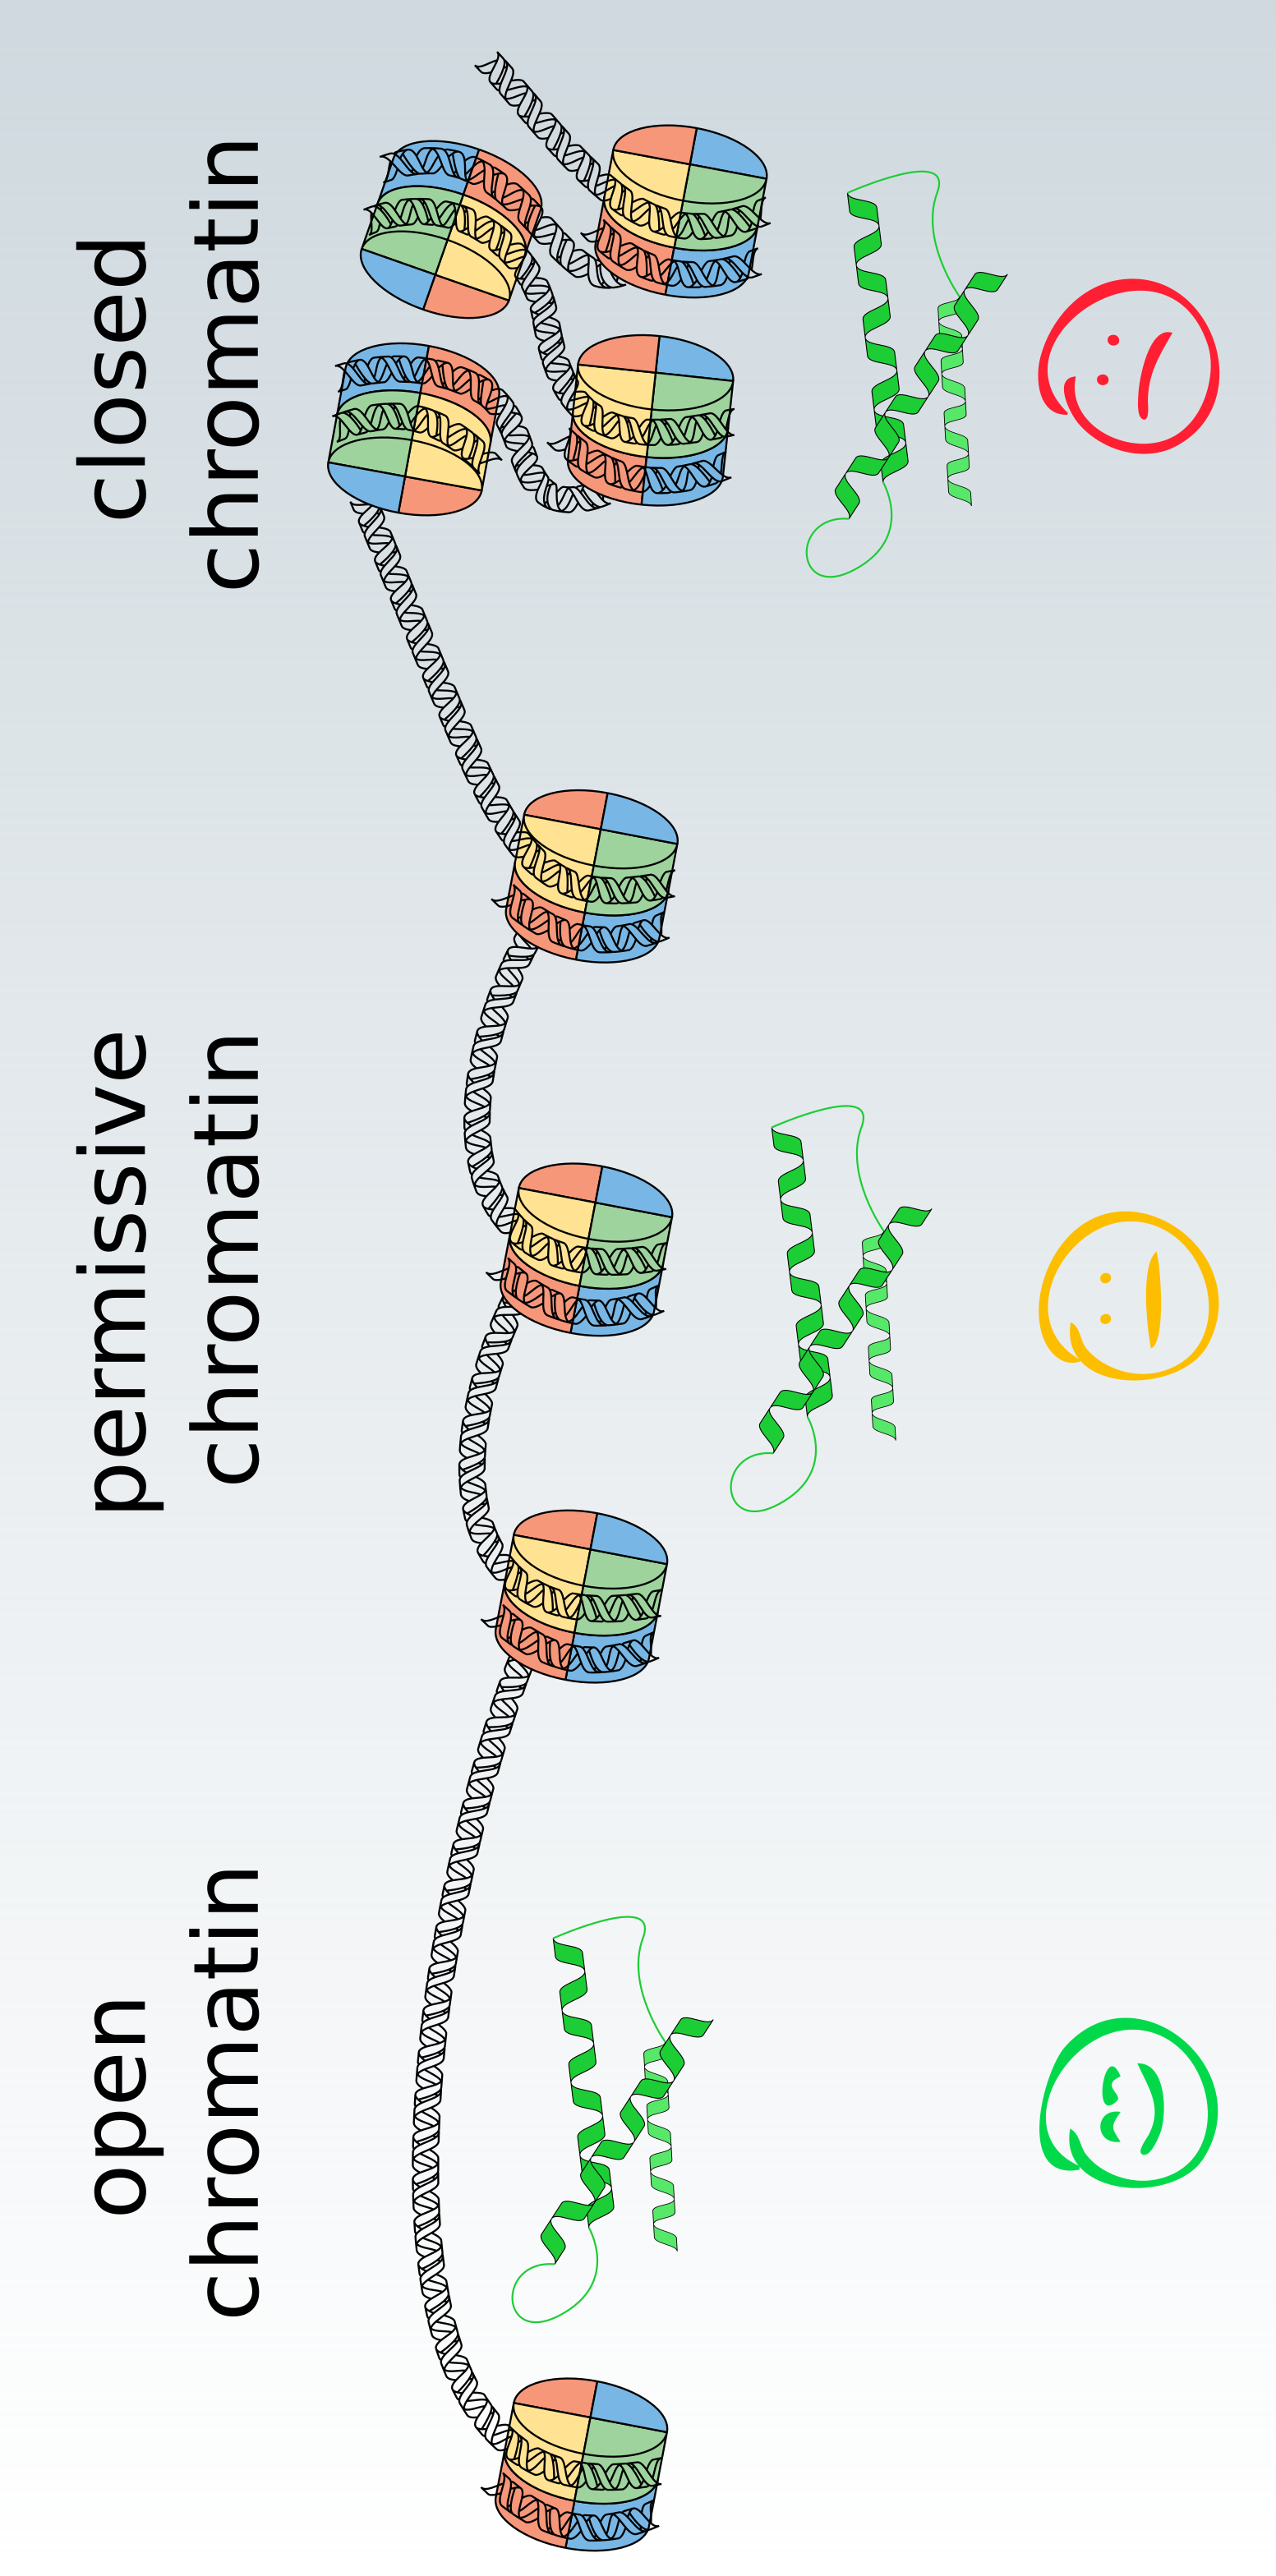
\includegraphics[height=0.9\textheight]{ch1.Introduction/imgs/accessibility.png}
    \caption{Caption}
    \label{fig:accessibility}
\end{figure}

\subsection{Transcription Factors}


\subsection{other regulatory modes}
% \subsubsection{mRNA degradation}
% \subsubsection{Post-transcriptional modification}
% \subsubsection{RNA transport}
% \subsubsection{Signal transduction}
\subsection{Gene regulatory networks}

\begin{figure}[H]
    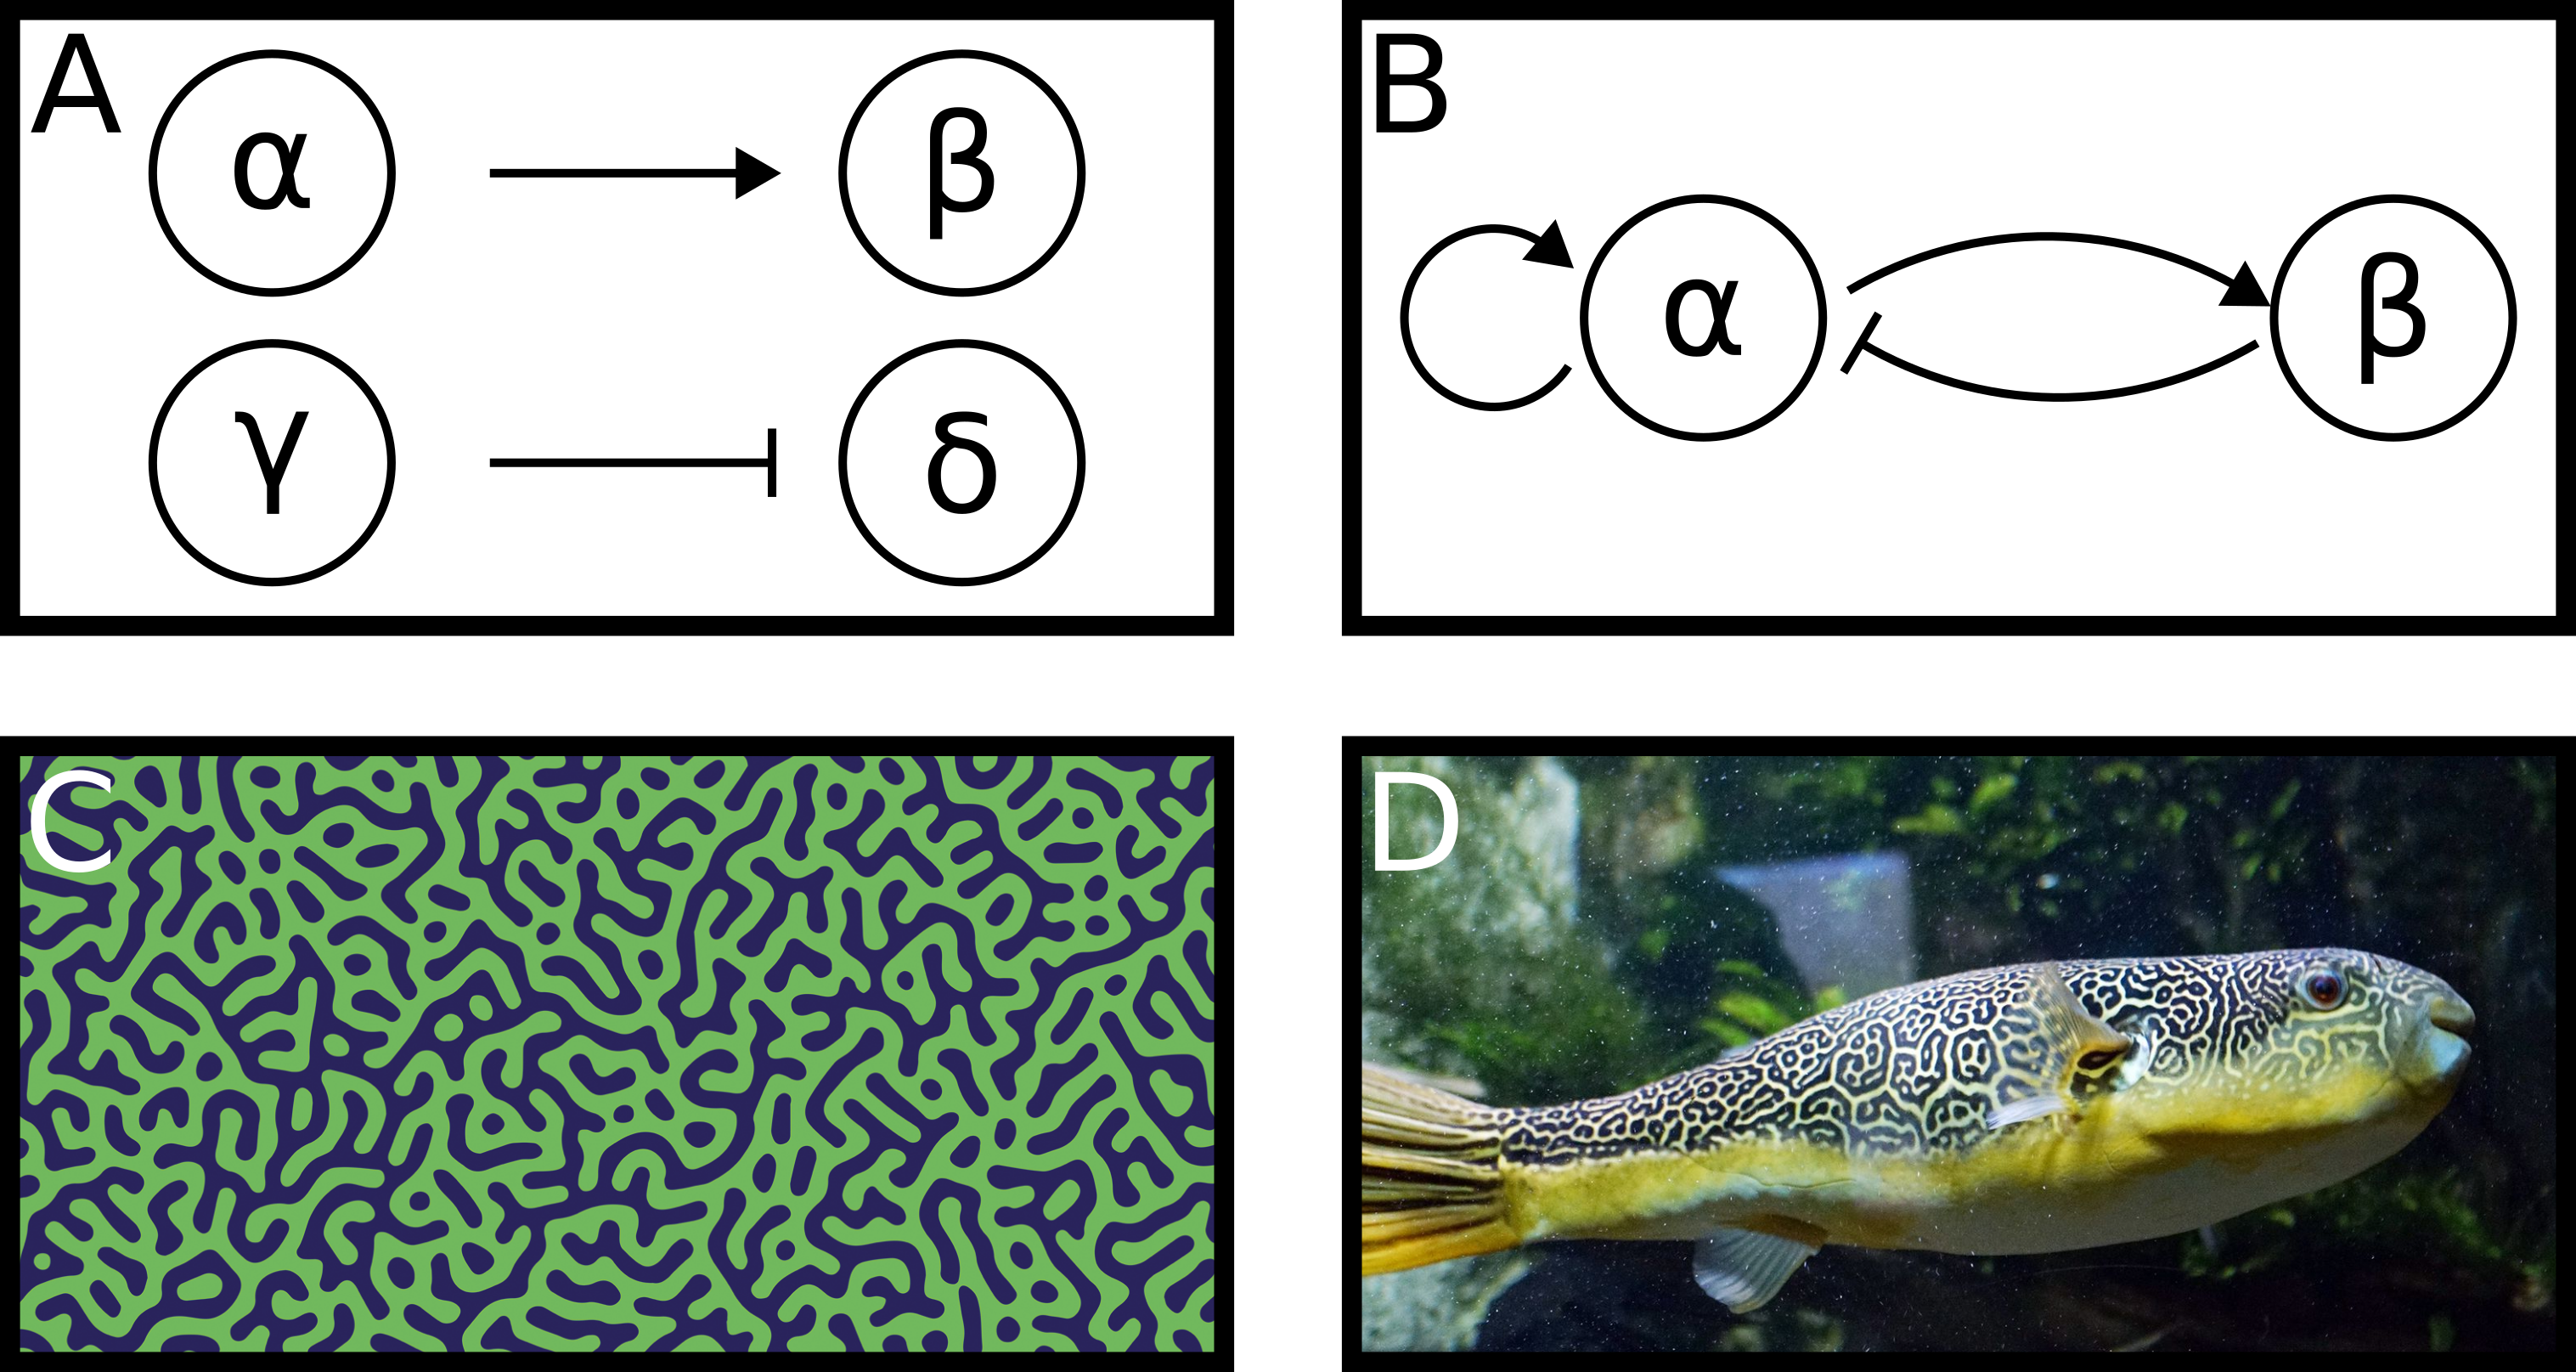
\includegraphics[width=\linewidth]{ch1.Introduction/imgs/network.png}
    \caption{https://en.wikipedia.org/wiki/Mbu\_pufferfish\#/media/File:Tetraodon\_mbu\_2.jpg}
    \label{fig:network}
\end{figure}

\section{Evolution}

\begin{figure}[H]
    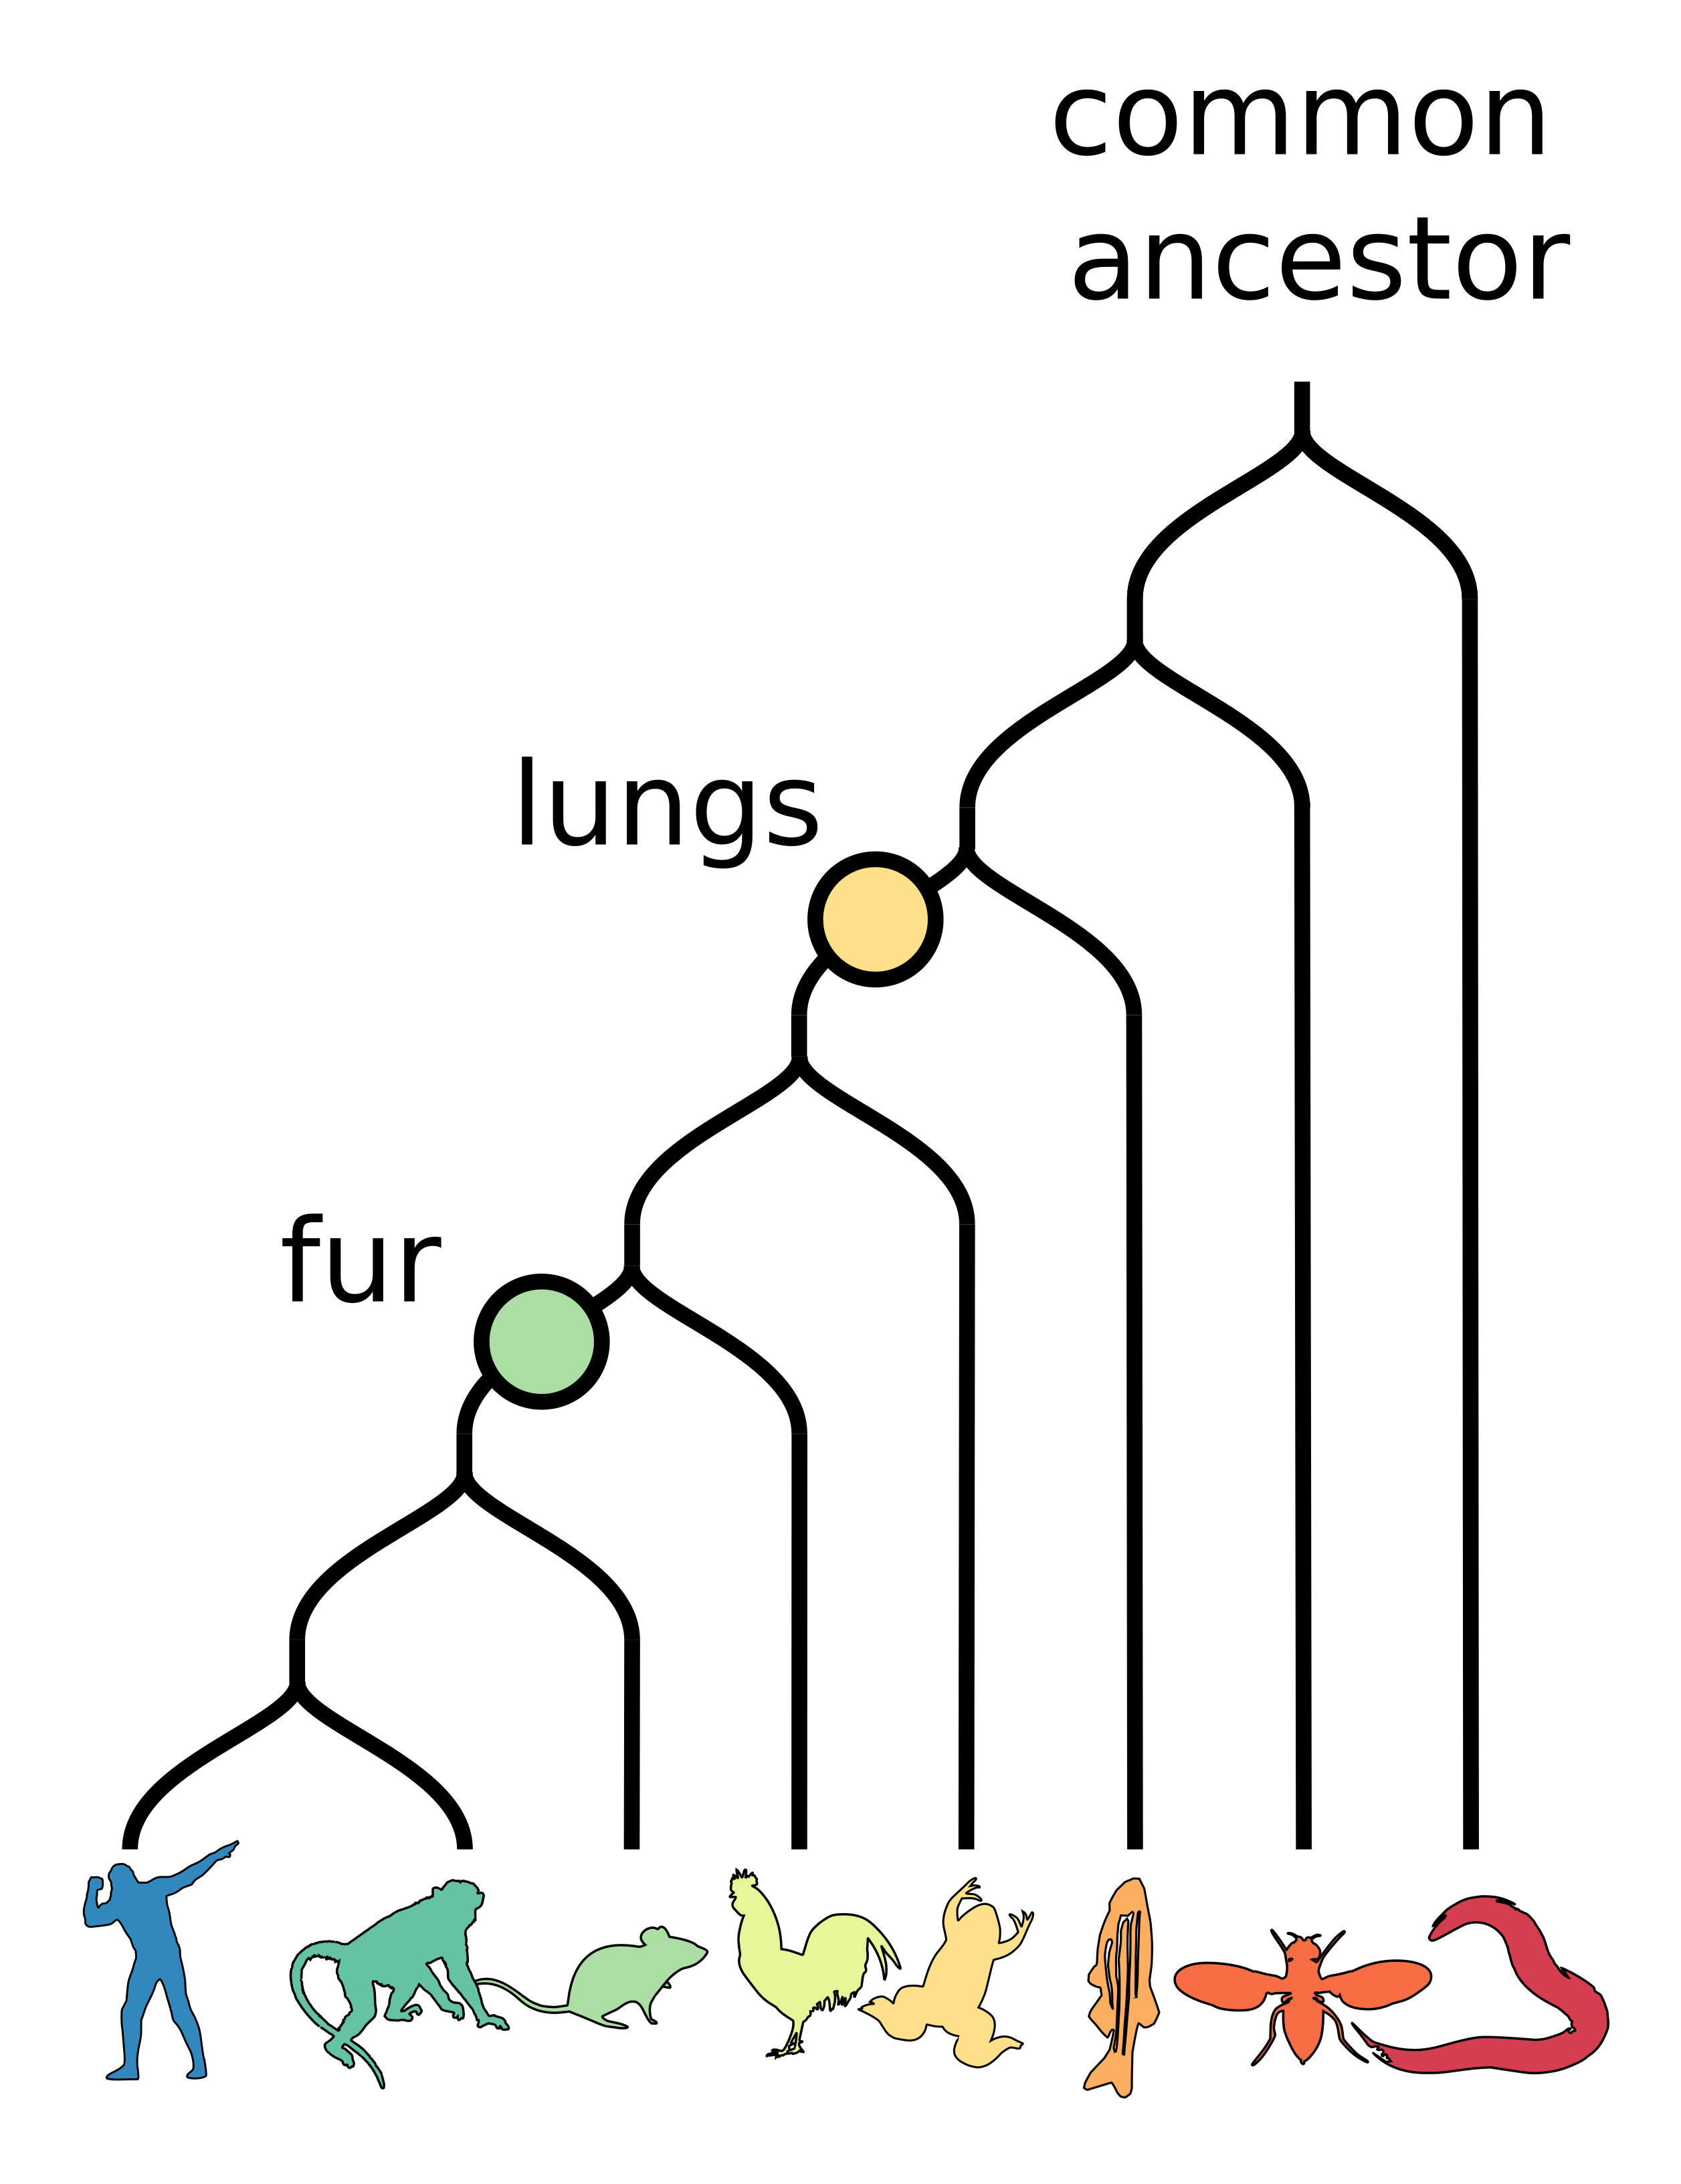
\includegraphics[width=0.5\linewidth]{ch1.Introduction/imgs/phylogeny.png}
    \caption{caption}
    \label{fig:phlogeny}
\end{figure}

\section{Development}

\section{Evolutionary development (evo-devo)}
\subsection{evo-devo gene toolkit}
\subsection{hox genes}

\section{Genomic analysis}

\begin{figure}[H]
    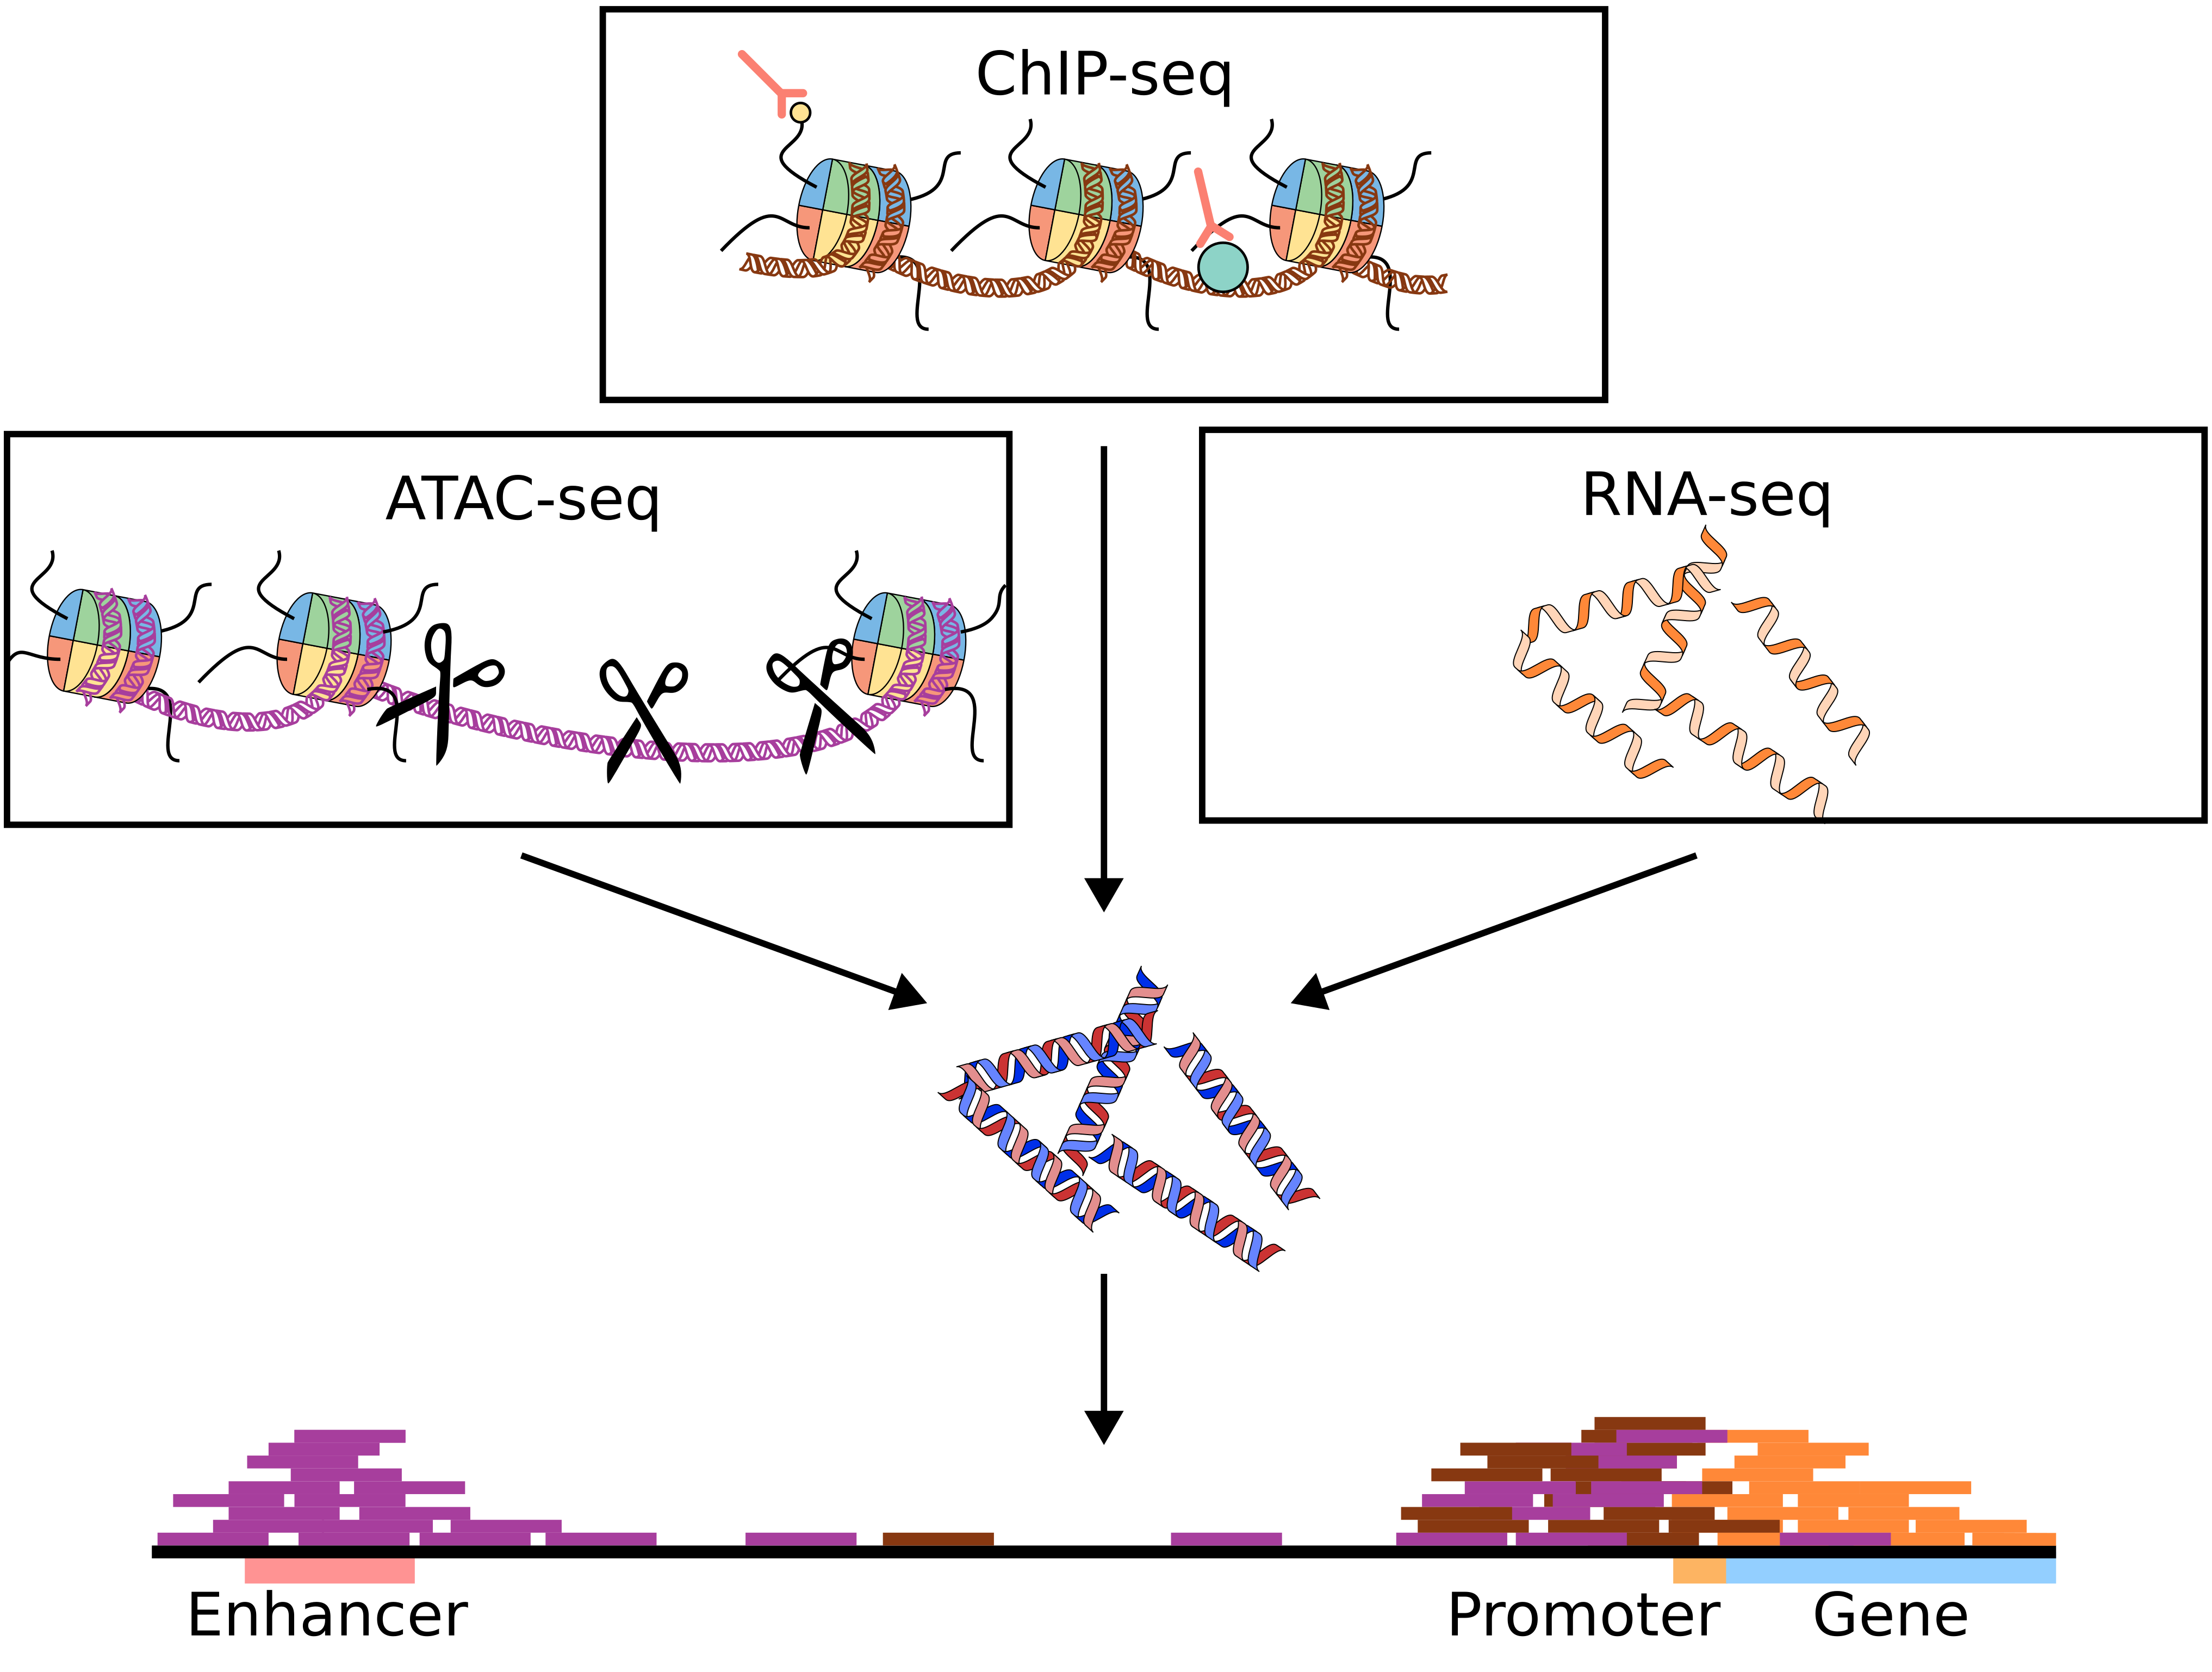
\includegraphics[width=\linewidth]{ch1.Introduction/imgs/analysis.png}
    \caption{caption}
    \label{fig:phlogeny}
\end{figure}

\section{Thesis overview}
